\subsection{Electromagetic Calorimeters}

 Energy of scattered electron are completely deposited in Calorimeters after electromagetic the cascade, so the goal of calibration is to relate the ADC signals collected by lead glass blocks in two layers of each Calorimeters to central momentum of scattered electrons (P0). A new variable E/P is defined as a ratio of cluster-reconstructed energy sum of calorimeters and P0, and it should be close to one if ADC channels are well calibrated.


 Due to the difference of two calorimeters, different methods were used to perform the calibrations on each arm. A minimization method was used to calibrate Shower and Preshower\cite{shower_ak}, and the Chi-Square is defined as: 
\begin{equation}
 \chi^{2} = \sum_{i=1}^{N}[\sum_{j\in M_{ps}^{i}}C_{j}\cdot (ADC_{j}^{i}-Ped_{j})+\sum_{k\in M_{sh}^{i}}C_{k}\cdot (ADC_{k}^{i}-Ped_{k})-P_{kin}^{i}]^{2}
\end{equation}

where \emph{i} is the \emph{i-th} event; \emph{j} is the \emph{j-th} preshower block while \emph{k} is the \emph{k-th} shower block;$M_{ps}^{i}$ and $M_{sh}^{i}$ are sets of preshower and shower included in the reconstructed cluster in the \emph{i-th} event; $ADC_{j/k}^{i}$ and $Ped_{j/k}$ respectively represent the ADC channel and mean pedestal value of a preshower or shower block in a certain event \emph{i}; $P_{kin}^{i}$ is the particle momentum in the \emph{i-th} event; and $C_{j/k}$ is a fitting paramter of a block which will be the gain factor of each ADC channel.

 To obtain the best results of fitting, electron samples are selected from data taken at the kinematics region of Quasi-Elastic tail where scattered electrons uniformly distribute along calorimeter blocks. A Fumili minimization package \cite{shower_luhj} is called to minimize the Chi-Square. The improvement after the calibration can be seen from Fig~\ref{pssh_cali}, where electrons are better separated from backgrounds, and  E/P is well centered at one. 

%\clearpage
\parbox[t]{0.45\textwidth}{
 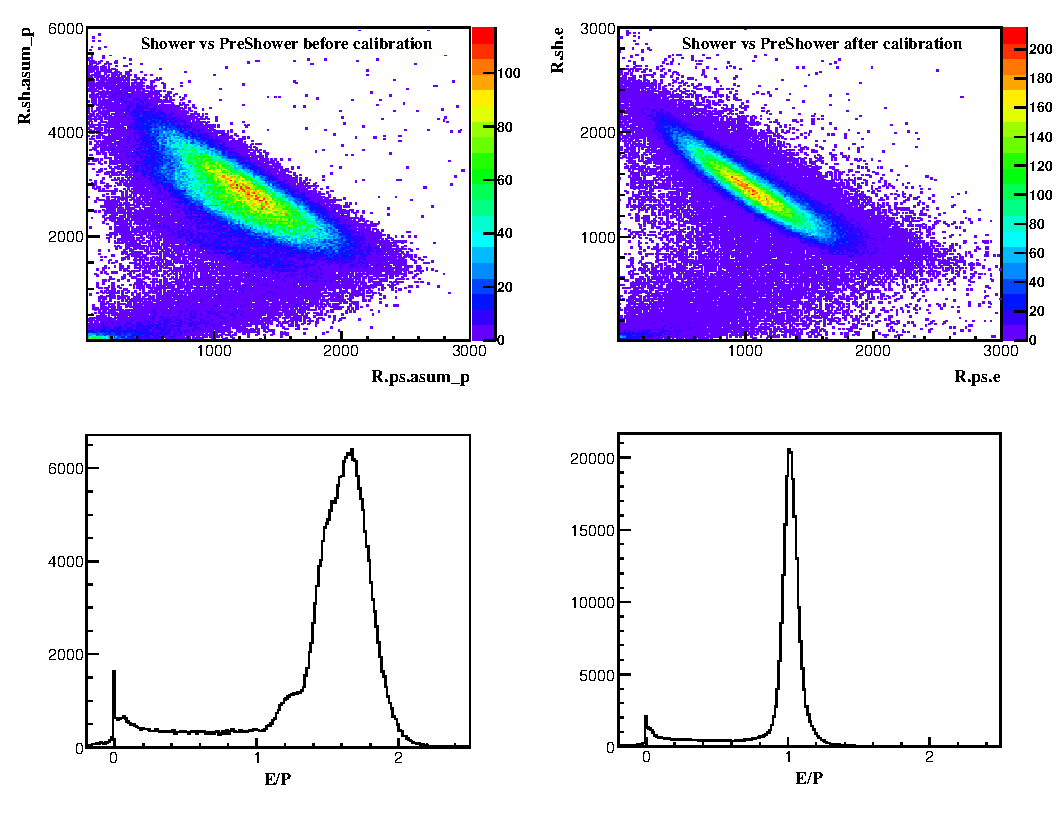
\includegraphics[width=\linewidth]{figures/calo/SH_Calibration.eps}
 \captionof{figure}{\footnotesize{Shower and PreShower calibration}}
 \label{pssh_cali}
}
\hfill
\parbox[t]{0.45\textwidth}{
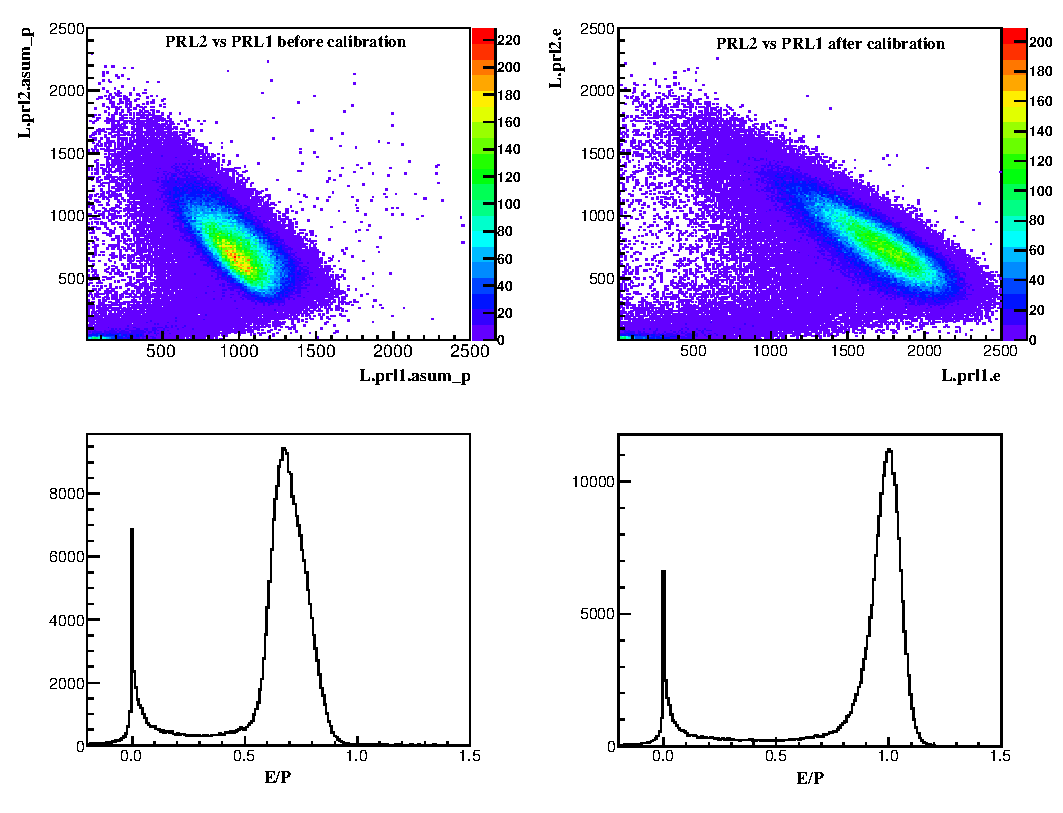
\includegraphics[width=\linewidth]{figures/calo/PRL_Calibration.eps}
\captionof{figure}{\footnotesize{PRL1 and PRL2 calibration}
\label{prl_cali}}
}

 Similar to the technique of Cherenkov detectors calibration, we aligned the minimum ionization peak in each block of pion rejectors using the cosmic ray data. The advantage of using cosmic ray data for the calibration is that the events uniformly distribut along the detector planes and the energy of particles from cosmic ray, mostly muon, deposited in lead glass blocks should be identical. We located the pedestal peak and muon peak in each ADC spectrum, and align the distance between themto be 100, by applying a gain factor defined as:
\begin{equation}
 C_{i} = \frac{100}{ADC_{i}^{muon}-ADC_{i}^{pedestal}}
\end{equation}

After aligning all ADCs of lead glass blocks, we calculated E/P with new obtained gain factors and did a final correction to shfit the peak to one:
\begin{equation}
 C_{i}^{real} = C_{i} \times \frac{1}{M_{E/P}}
\end{equation}

where $M_{E/P}$ represents the mean value of the E/P peak. The quality of the calibration can be checked from Fig ~\ref{prl_cali}.

 The stability of Calorimeters calibration is checked from Fig~\ref{calo_stability} and resolutions of calibration are extracted. The resolution of calorimeters is 2.53\% per GeV on HRS-R and 3.21\% per GeV on HRS-L, where the one on HRS-L is slightly worse than the one on HRS-R is due to the fact that Pion Rejectors are not total absorbers.

\begin{figure}[ht]
  \includegraphics[width=0.45\linewidth]{figures/calo/R_Calo_Align_new.eps}
  \hfill
  \includegraphics[width=0.45\linewidth]{figures/calo/L_Calo_Align_new.eps}
  \caption{\footnotesize{Calorimeter calibration stability and resolution}}
  \label{calo_stability}
\end{figure}
